\clearpage
\newpage

\subsubsection{Estensione A: Disattivazione Notifiche dalla Visualizzazione di una Notifica}

Per offrire un maggiore controllo sulla gestione delle notifiche senza interrompere l’esperienza utente, il sistema permette di disattivare una categoria direttamente dalla visualizzazione di una notifica specifica. Questa variante è progettata per garantire una modifica consapevole delle preferenze, evitando azioni impulsive che potrebbero compromettere la ricezione di informazioni rilevanti.

\vspace{0.5cm}
\subsubsection{Interfaccia e Comportamento del Bottone}
Alla fine del testo di ogni notifica, se la relativa categoria è attiva, è presente un pulsante neutro con la dicitura “Disattiva notifiche”. Accanto al pulsante, un testo in grigio informa l’utente della funzione del pulsante, evitando ambiguità. L’utilizzo di colori non accesi e di un design discreto segue il principio della \textbf{gerarchia visiva} \cite{pieters2004}, scoraggiando azioni impulsive che potrebbero portare alla perdita involontaria di notifiche future.

\vspace{0.5cm}
\subsubsection{Modifica dello Stato e Feedback Visivo}
Quando l’utente clicca sul pulsante, il testo del pulsante cambia colore, diventando rosso, e il messaggio a fianco si aggiorna per sottolineare che la categoria di notifiche è stata disattivata. Questo utilizza il principio della \textbf{salienza visiva} \cite{nielsen1995}, enfatizzando il cambiamento e rendendo immediatamente chiara la conseguenza dell’azione.

\vspace{0.5cm}
\subsubsection{Incentivo alla Riattivazione}
Una volta disattivata una categoria tramite questa modalità, viene visualizzato un secondo pulsante con una call-to-action mirata per incentivare la riattivazione delle notifiche. Il design e il posizionamento del pulsante sfruttano il \textbf{principio dell’affordance} \cite{norman1988}, rendendo chiaro che l’utente ha la possibilità di tornare indietro sulla sua decisione in modo semplice e immediato.
\newline
Questa estensione si integra perfettamente con il modello generale di gestione delle notifiche, garantendo un’interazione fluida e coerente con le esigenze dell’utente. Nel caso in cui l’utente scelga di riattivare la categoria delle notifiche direttamente da una notifica, si passa all’\textbf{Estensione F}, che approfondisce questa modalità di gestione a partire dalle notifiche disattivate.
\begin{figure}[ht]
    \centering
    \begin{tikzpicture}[node distance=1.5cm and 1cm, auto]
        % Nodo per immagine 1 con didascalia sotto
        \node (img1) {
            \begin{tabular}{c}
                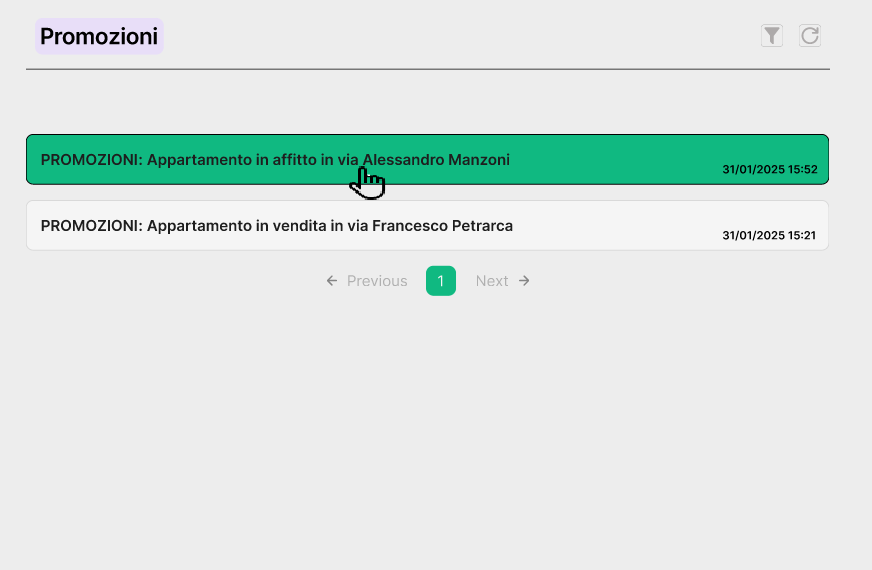
\includegraphics[width=0.4\textwidth]{Immagini/Mockup/notifiche/estensione A/clickNotifica.png} \\
                Cockburn: Extension A.2/A.3
            \end{tabular}
        };
        
        % Nodo per immagine 2 con didascalia sotto, posizionato a destra di img1
        \node (img2) [below=of img1] {
            \begin{tabular}{c}
                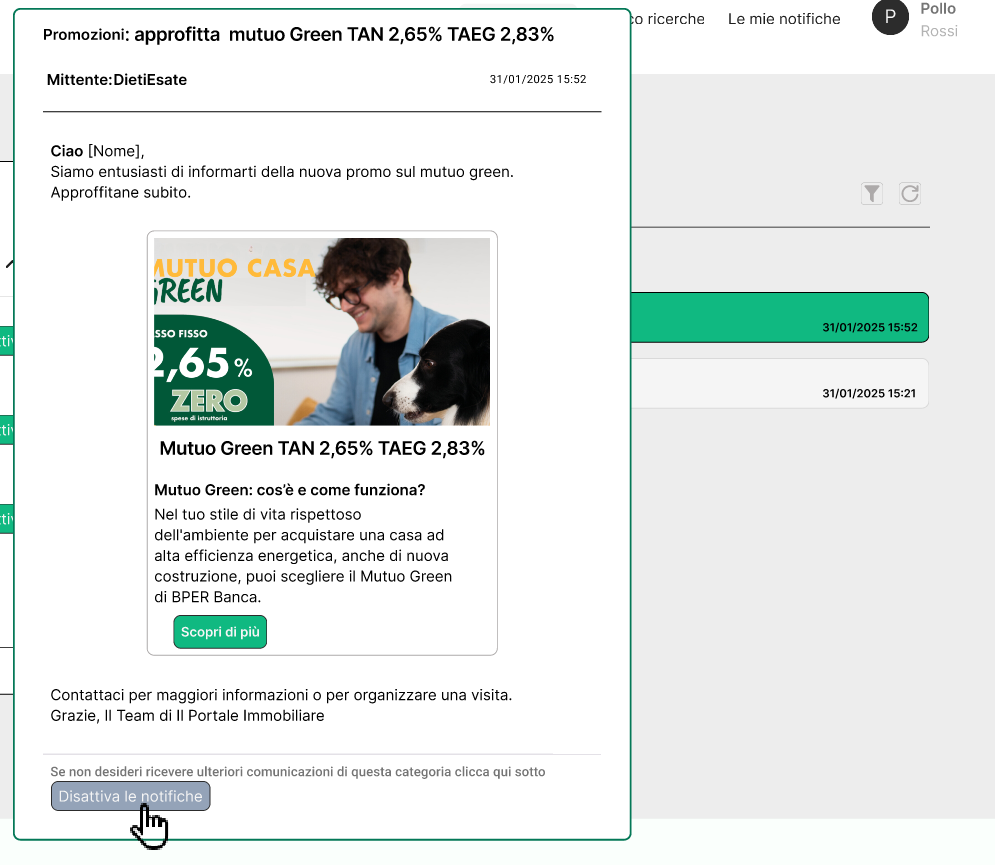
\includegraphics[width=0.4\textwidth]{Immagini/Mockup/notifiche/estensione A/clickDisattiva.png} \\
                Cockburn: Extension A.4
            \end{tabular}
        };
        
        % Nodo per immagine 3 con didascalia sotto, posizionato sotto img2
        \node (img3) [below=of img2] {
            \begin{tabular}{c}
                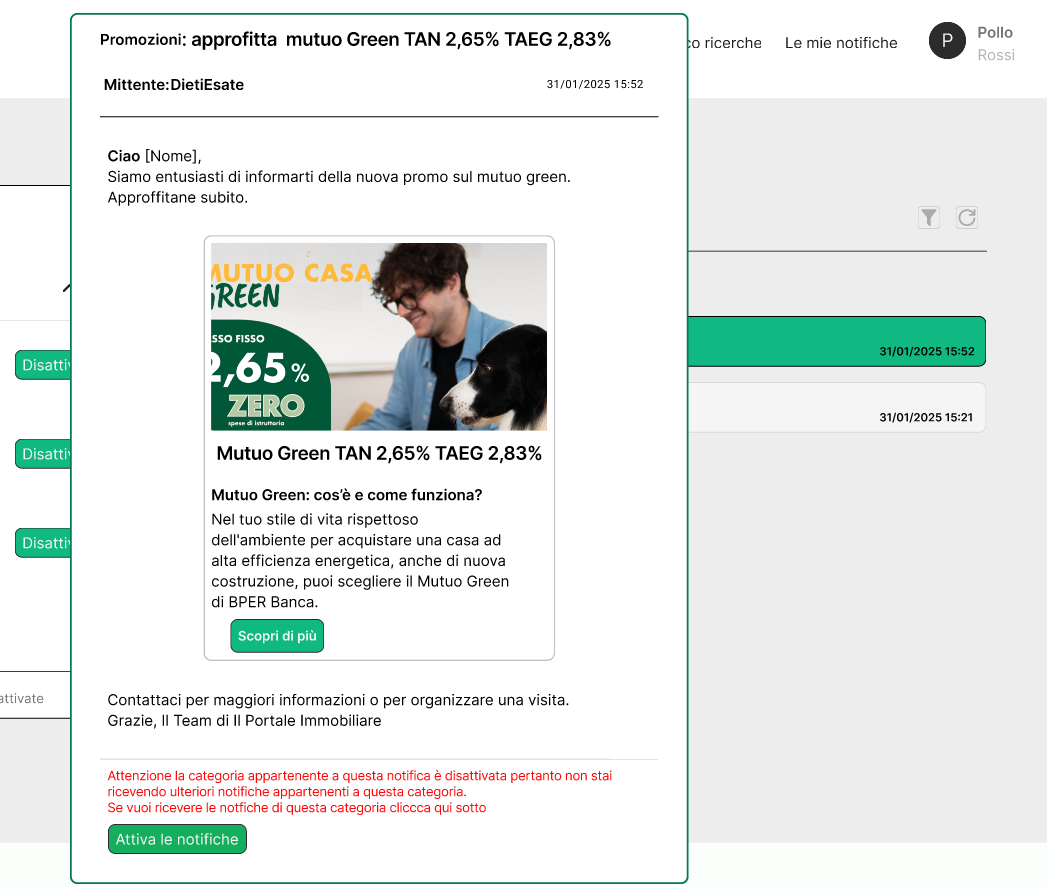
\includegraphics[width=0.4\textwidth]{Immagini/Mockup/notifiche/estensione A/disattivato.png} \\
                Cockburn: extension A.5
            \end{tabular}
        };
        
        % Disegna le frecce
        \draw[->, thick] (img1) -- (img2);
        \draw[->, thick] (img2) -- (img3);
      
    \end{tikzpicture}
    \caption{Mockup: estensione A della tabella di Cockburn del caso d'uso disattiva/attiva categoria notifica}
    \label{fig:mockup_estensione_A_disattiva_notifiche}
\end{figure}

\newpage

